%========================================================================================
% TU Dortmund, Informatik Lehrstuhl VII
%========================================================================================

\chapter{Graphische Ausgabe}
\label{Kapitel 2}
%
In der graphischen Ausgabe der Anwendung sollen alle Objekte dargestellt werden. Zu den darstellbaren Objekten gehören der Ball, der Schläger, das Spielfeld und eine Zielscheibe, wie in Abbildung \ref{fig:gameScene} zu sehen ist.

\begin{figure}[h]
	\centering
	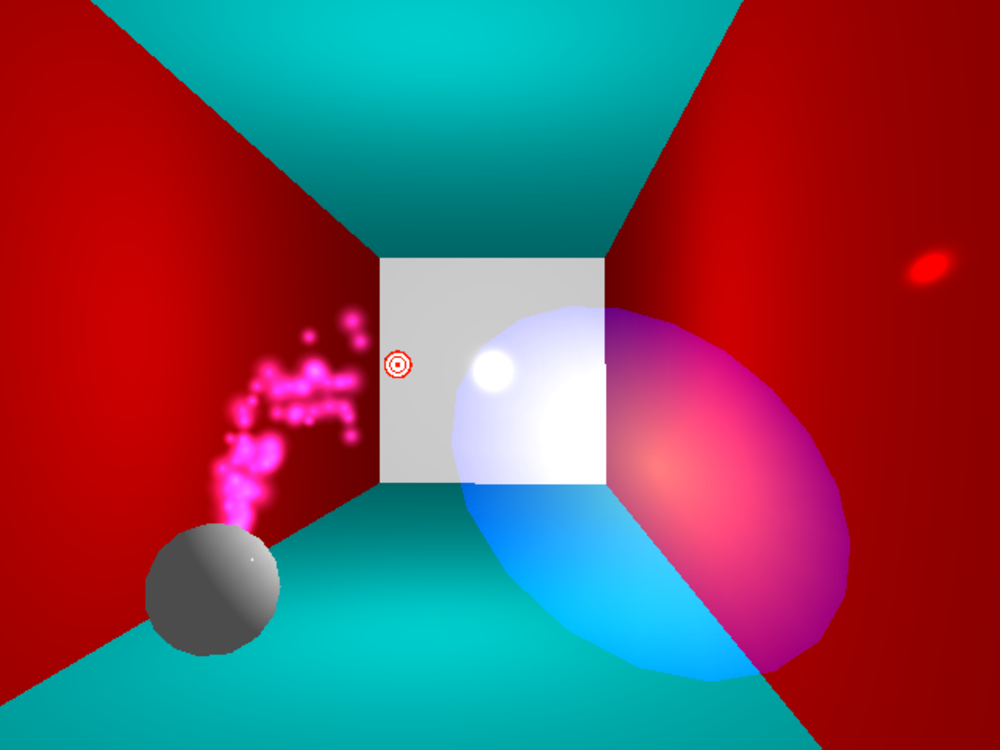
\includegraphics[width=0.6\linewidth]{bilder/gameScene}
	\caption{Szene aus der Anwendung}
	\label{fig:gameScene}
\end{figure}


\section{Rendering Architektur}
\label{Kapitel_2_-_Unterkapitel_1}
%
Der in Abbildung \ref{fig:renderingSystem} dargestellte Ausschnitt des Klassendiagramms (siehe Anhang \ref{anhangA}) zeigt die zentralen Klassen des Rendering-Systems und ihre Beziehungen zueinander.

\begin{figure}[h]
	\centering
	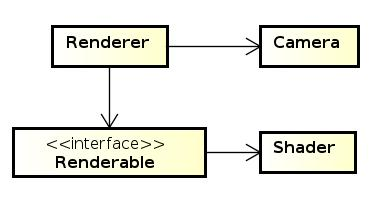
\includegraphics[width=0.6\linewidth]{bilder/RenderingSystem}
	\caption{Klassen des Rendering-Systems}
	\label{fig:renderingSystem}
\end{figure}

Die Klassen, die die Spielobjekte repräsentieren, also {\texttt{Ball}}, {\texttt{Racket}}, {\texttt{Box}} und {\texttt{Scorefield}}, enthalten Member, die das {\texttt{Renderable}}-Interface implementieren und für die graphische Darstellung zuständig sind. Die Klassen die das Interface implementieren sind:

\begin{itemize}
	\setlength\itemsep{0.05em}
	\item {\texttt{BallRenderable}} und {\texttt{BallParticleRenderable}} für den Ball
	\item {\texttt{RacketRenderable}} für den Schläger
	\item {\texttt{BoxRenderable}} für das Spielfeld
	\item {\texttt{ScorefieldRenderable}} für die Zielscheibe 	
\end{itemize}

Jedes dieser Renderables kümmert sich bei der seiner Initialisierung um die Erzeugung der Render-Daten, der Buffer, die die Render-Daten halten, und des Shader-Programms. Der Renderer selbst hält ein {\texttt{Camera}}-Objekt und eine Liste der Renderables und delegiert den Render-Call aus der Hauptschleife an die einzelnen Renderables. Dabei wird das {\texttt{Camera}}-Objekt an die Renderables übergeben, sodass diese sich die View- und Projection-Matrix holen können. Bei der Aktualisierung eines Spielobjekts in der Hauptschleife gibt das Spielobjekt die neuen Daten an sein Renderable weiter, damit dieses die Model-Matrix aktualisieren kann. Eine Ausnahme bildet das {\texttt{BallParticleRenderable}}, das für jedes Partikel eine eigene Model-Matrix erzeugen muss und in Abschnitt \ref{Kapitel_2_-_Unterkapitel_2} genauer erläutert wird.

\section{3D-Modelle der Renderables}
%
Für das Erstellen der Modelle, die in der Anwendung zu sehen sind, wurde keine Modelling-Software verwendet. Da es sich bei den Modellen um einfache geometrische Objekte wie Kugeln, Kreise, und Rechtecke handelt, werden die Render-Daten, also Vertizes, Normale, Farben und ggfs. Indizes für die Faces, innerhalb der Renderables erzeugt.

\subsection{Spielfeld}
%
In der graphischen Ausgabe hat das Spielfeld die Form eines Quaders. Intern werden die einzelnen Wände als Ebenen repräsentiert. Da die {\texttt{Plane}}-Klasse eine Ebene in der Hesseschen Normalform\footnote{Näheres dazu in Kapitel \ref{Kapitel 4}} abspeichert, können aus den Abstandswerten der einzelnen Ebenen leicht die Koordinaten für die 8 Vertices des Modells gewonnen werden.

\subsection{Schläger}
%
Der Schläger ist in der graphischen Ausgabe ein regelmäßiges Polygon. Daher reduziert sich das Problem der Erzeugung der Vertices auf die Berechnung von Koordinaten auf dem Einheitskreis. Algorithmus \ref{algo_circle} enthält einen Ausschnitt aus dem Programmcode als Pseudocode.

\begin{algorithm}[t]
	\centering
	\caption{Algorithmus für die Erzeugung des Schläger-Modells} \label{algo_circle}
	\begin{algorithmic}
		\REQUIRE Anzahl der Kreissektoren $s$
		\ENSURE Vertices $V$
		\STATE $\Delta\theta := 2*\pi/s$
		\STATE new Array $V[s+1]$
		\STATE $V[0] := (0,0,0)$
		\FOR{$i := 0$ \TO $i < s$}
		\STATE $V[i+1] := (\cos(i*\Delta\theta), \sin(i*\Delta\theta), 0)$
		\ENDFOR
	\end{algorithmic}
\end{algorithm}

Für ein besseres visuelles Ergebnis lässt sich über den Parameter $s$ die Anzahl der Vertices steuern, um das Schläger-Modell mehr nach einem Kreis aussehen zu lassen. In der Anwendung besteht Das Schläger-Modell aus 21 Vertices.

\subsection{Ball}
%
Die Erzeugung der Vertices für das Ball-Modell lässt sich sich auf die Berechnung von Koordinaten auf der Kugeloberfläche der Einheitskugel zurückführen. Das Modell wird dabei in die beiden Pole und eine bestimmte Anzahl an Ringen, auf denen sich Vertices befinden, geteilt. Jeder Ring hat dabei die gleiche Anzahl an Vertices. Algorithmus \ref{algo_sphere} enthält einen Ausschnitt des Programmcodes als Pseudocode.

\begin{algorithm}[t]
	\centering
	\caption{Algorithmus für die Erzeugung des Ball-Modells} \label{algo_sphere}
	\begin{algorithmic}
		\REQUIRE Anzahl der Ringe $r$, Anzahl der Punkte pro Ring $p$
		\ENSURE Vertices $V$
		\STATE $\Delta\phi := 2*\pi/p$
		\STATE $\Delta\theta := \pi/(s + 1)$
		\STATE $\phi := 0$
		\STATE $\theta := 0$
		\STATE new Array $V[2 + r * p]$
		\STATE $V[0] := (0,0,1)$
		\STATE $V[1 + r * p] := (0,0,-1)$
		\STATE $offset := 0$
		\FOR{$i := 1$ \TO $i \leq r$}
		\STATE $\theta := \theta +\Delta\theta$
			\FOR{$j := 0$ \TO $j < p$}
			\STATE $\phi := \phi +\Delta\phi$
			\STATE $V[i + j + offset] := (\sin(\theta)*\cos(\phi), sin(\theta) * \sin(\phi), \cos(\theta))$
			\ENDFOR
			\STATE $\phi := 0$
			\STATE $offset := offset + p - 1$
		\ENDFOR
	\end{algorithmic}
\end{algorithm}

Auch hier lässt dich mit höheren Werten für die Parameter $p$ und $r$ ein besseres visuelles Ergebnis erzielen. In der Anwendung hat das Ball-Modell 15 Ringe mit jeweils 10 Vertices, also insgesamt 152 Vertices.

\iffalse
\begin{figure}[h]
	\centering
	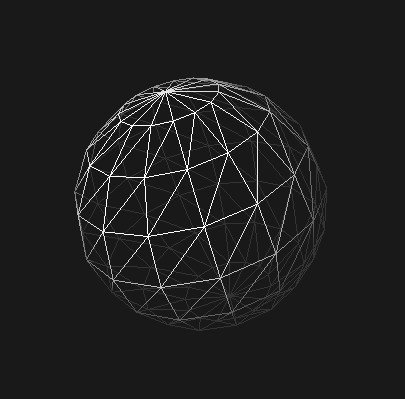
\includegraphics[width=0.5\linewidth]{bilder/ballWireframe}
	\caption{Ball im Wireframe}
	\label{fig:ballWireframe}
\end{figure}
\fi

\section{Kamerabewegung}
%
Um die Flugbahn des Balles besser einschätzen zu können und um ein besseres Gefühl für die
Position des Schlägers innerhalb des Spielfeldes zu erhalten, bewegt sich die Kamera bei Bewegung des Schlägers mit. Die Kamerabewegung ist in Abbildung \ref{fig:camera} dargestellt.

\begin{figure}[t]
	\centering
	\subfigure[Kamera in neutraler Position]
	{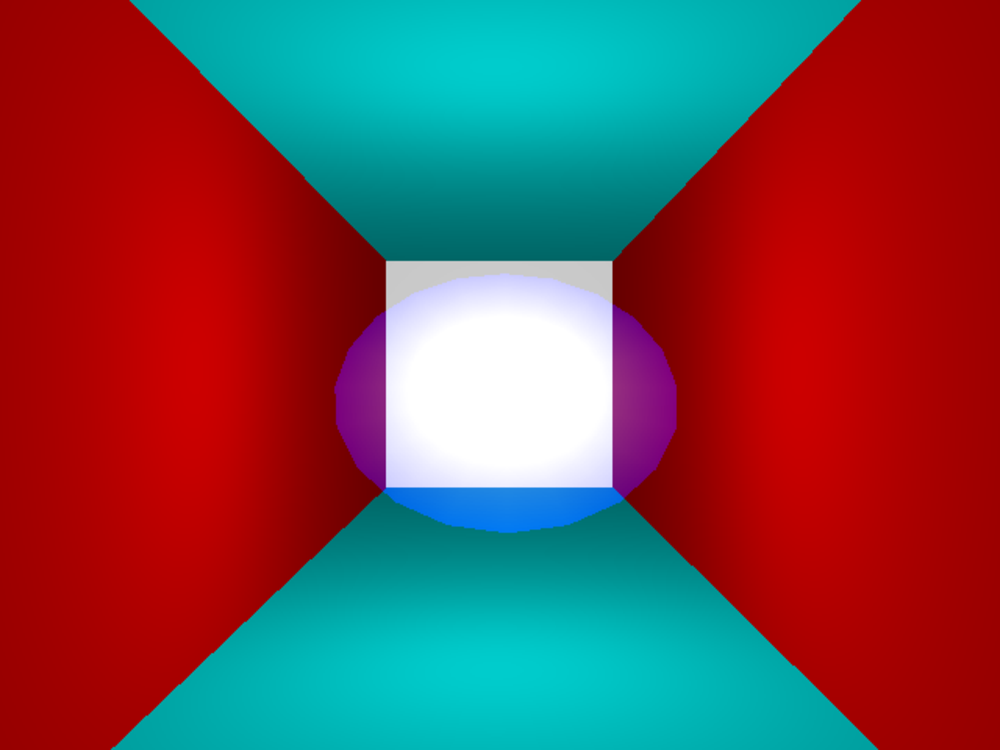
\includegraphics[scale=0.4]{bilder/cameraNeutral}\label{fig:cameraNeutral}
	}
	\vspace{1.5cm}%
	\subfigure[Kamera bei Bewegung des Schlägers nach rechts oben]
	{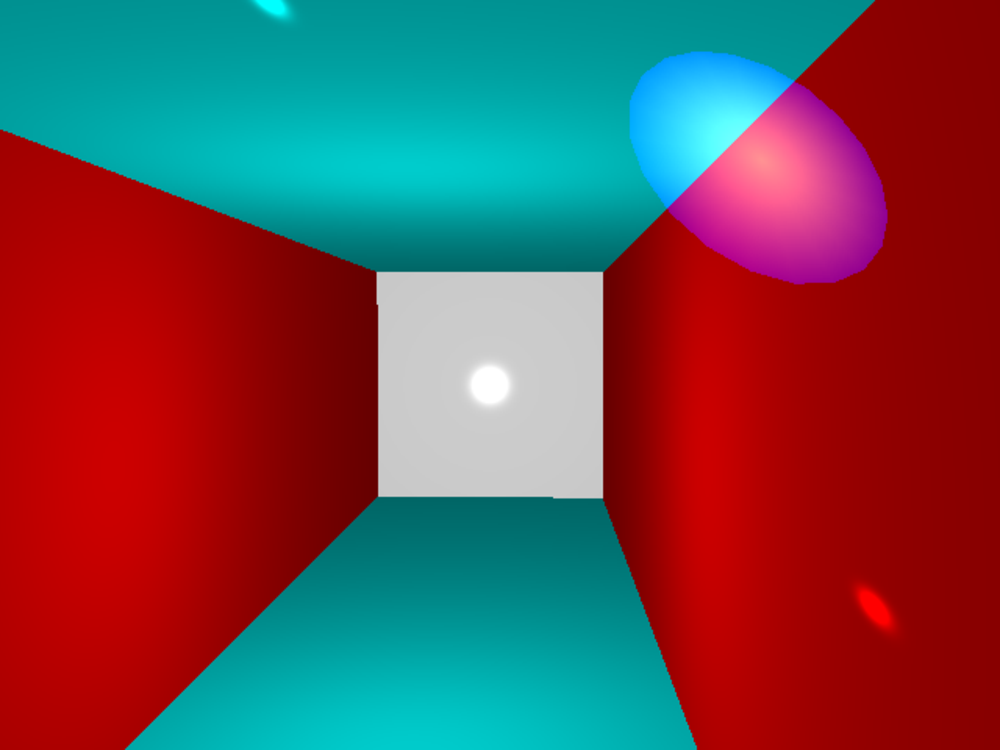
\includegraphics[scale=0.4]{bilder/cameraMoved}\label{fig:cameraMoved}
	}
	\vspace{-1.5cm}
	\caption[Weitere Testbilder]{Kameraposition bei Bewegung des Schlägers}
	\label{fig:camera}
\end{figure}

In jedem Durchlauf der Hauptschleife wird der Kamera nach dem Aktualisieren der Position des Schlägers die neue Position mitgeteilt, wobei nur die $x$- und $y$-Koordinate in die neue Kameraposition mit einfließen. Die Kamera passt dann die View-Matrix an. Der Bewegungsbereich der Kamera ist so eingeschränkt, dass , wenn der Schläger außerhalb dieses Bewegungsbereiches bewegt wird, die Kamera innerhalb des Spielfelds verbleibt.
\section{Partikelsystem}
\label{Kapitel_2_-_Unterkapitel_2}
%
Partikelsysteme sind in interaktiven Anwendungen wie Computerspiele und in der Postproduktion von Filmen, seien es Real- oder Animationsfilme, allgegenwärtig.
Man denke an typische Effekte wie Feuer und Rauch, aber auch Flüssigkeiten lassen sich mithilfe von Partikelsystemen realisieren.

Nach \cite{reeves:particle_systems} sind Partikelsysteme besonders geeignet für Objekte die sich aufgrund ihrer Komplexität nur schwer mit einem Mesh darstellen lassen und sich im Verlauf der Zeit in ihrer Form ändern. Eine einfache Repräsentation solcher Objekte lässt sich daher mit Wolken aus Partikeln umsetzen, wobei die Partikel einfache Primitive wie Punkte, Linien und Dreiecke sind\cite{reeves:particle_systems}.

In der Anwendung wird ein Partikelsystem genutzt um den Flugverlauf des Balles darzustellen. Dabei sind die Partikel Quads, bestehend aus jeweils 6 Vertices, auf die eine Textur projiziert wird.

\subsection{Komponenenten des Partikelsystems}
\label{Kapitel_2_-_Unterkapitel_2.1}
%
In der Anwendung besteht das Partikelsystem aus zwei Klassen, nämlich dem {\texttt{Particle}} und dem {\texttt{BallParticleRenderable}}.

Die {\texttt{Particle}} Klasse repräsentiert ein Partikel, welches eine Position in Weltkoordinaten, eine Geschwindigkeit, eine Lebensdauer und eine Größe hat. 
Die {\texttt{BallParticleRenderable}} Klasse ist für die Darstellung und Verwaltung aller im System vorhandenen Partikel zuständig. Zur Verwaltung gehört das emittieren neuer Partikel, das Aktualisieren der aktiven Partikel und Löschen der ‚toten‘ Partikel, also solcher, deren Lebensdauer null erreicht hat. Die Klasse hält Attribute, die die maximale Anzahl der aktiven Partikel beschränkt sowie die Emittiergeschwindigkeit.  Sie hat auch ein Attribut für die Position. Alle neuen Partikel werden relativ zu dieser Position emittiert. Dabei ist die Position des Emittierpunktes auf dem Rand des Balles entgegengesetzt dem Geschwindigkeitsvektor des Balles. Da die Position des Emittierpunktes an die Position des Balles gekoppelt ist, wird bei jedem Update des {\texttt{Ball}}-Objekts die neue Position an den {\texttt{BallParticleRenderable}} weitergegeben.

\subsection{Instanced Rendering}
\label{Kapitel_2_-_Unterkapitel_2.2}
%
Instanced Rendering bezeichnet eine effiziente Variante des Renderns von Objekten die dieselben Renderdaten verwenden, sich aber nur darin unterscheiden, wo sie im Weltkoordinatensystem platziert werden. Für die Partikel des Partikelsystems trifft dies zu, da jedes Partikel, wie bereits erwähnt, ein einfaches Quad ist und sich nur in seiner Position und Größe unterscheidet.

Die Effizienz dieser Methode rührt daher, dass zum Rendern der Partikel nun nicht mehr über die Liste aller Partikel iteriert wird und für jedes Partikel ein Draw-Call getätigt wird. Stattdessen wird pro Frame nur ein einziger Draw-Call getätigt, das heißt, dass nur ein Befehl über den langsamen Peripheriebus zur Grafikkarte gesendet werden muss. Für das Instanced Rendering bietet OpenGL die Funktionen {\texttt{glDrawArraysInstanced}} und {\texttt{glDrawElementsInstanced}}.

Um nicht zu sehr in den technischen Details zu versinken, soll nur kurz schematisch anhand von Abbildung \ref{fig:vao} der Vorgang beim Rendern der Partikel erläutert werden.
%Todo vao bild;kurz auf performance eingehen; verweis auf super bible

\begin{figure}[h]
	\centering
	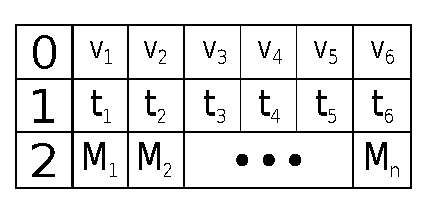
\includegraphics[scale=0.8]{bilder/vao}
	\caption{VAO im {\texttt{BallParticleRenderable}} nach jedem Update der Partikel}
	\label{fig:vao}
\end{figure}

Wie an Abbildung \ref{fig:vao} zu sehen ist, befinden sich die Vertizes $v_1\dotsc v_6$ , die Texturkoordinaten $t_1\dotsc t_6$ und die Model-Matrizen $M_1\dotsc M_n$, wobei $\mathnormal{n}$ die Anzahl der aktiven Partikel ist, in ihren eigenen Array-Buffer des VAOs des {\texttt{BallParticleRenderable}}-Objekts. Die Vertices und Texturkoordinaten ändern sich nicht. Die Model-Matrizen hingegen werden bei jedem Update der Partikel neu erzeugt und an den Array-Buffer gesendet.

Um Instanced Rendering zu nutzen muss der Array-Buffer der Model-Matrizen als Instance-Attribut des Vertex-Shaders deklariert werden. Dies sollte bei der Assoziation der Array-Buffer mit den Attributen des Vertex-Shader-Programms geschehen.
Beim Rendern einer Instanz werden nun alle Vertexdaten und Texturkoordinaten, die keine Instanz-Variablen sind, und die jeweilige Model-Matrix der Instanz verwendet.

Für weitere Informationen zum Thema Instanced Rendering sei auf \cite{ksls:2013} verwiesen.

\subsection{Blending und Tiefentest}
\label{Kapitel_2_-_Unterkapitel_2.3}
%
In dem verwendeten Partikelsystem sollen die Farben der Partikel, wenn sie sich überlagern, addiert werden. Der resultierende Effekt ist, dass bei genügend sich überlagernden Partikel ein leuchtend weißer Bereich zu sehen ist. Blending erlaubt es, Farben miteinander zu vermischen und ist ein Teil der Verarbeitung der Fragmente in der Rendering Pipeline. OpenGL bietet verschiedene Blending-Arten an, die durch den Aufruf der Funktion {\texttt{glBlendFunc}} eingestellt werden können. 

\begin{figure}[h]
\centering
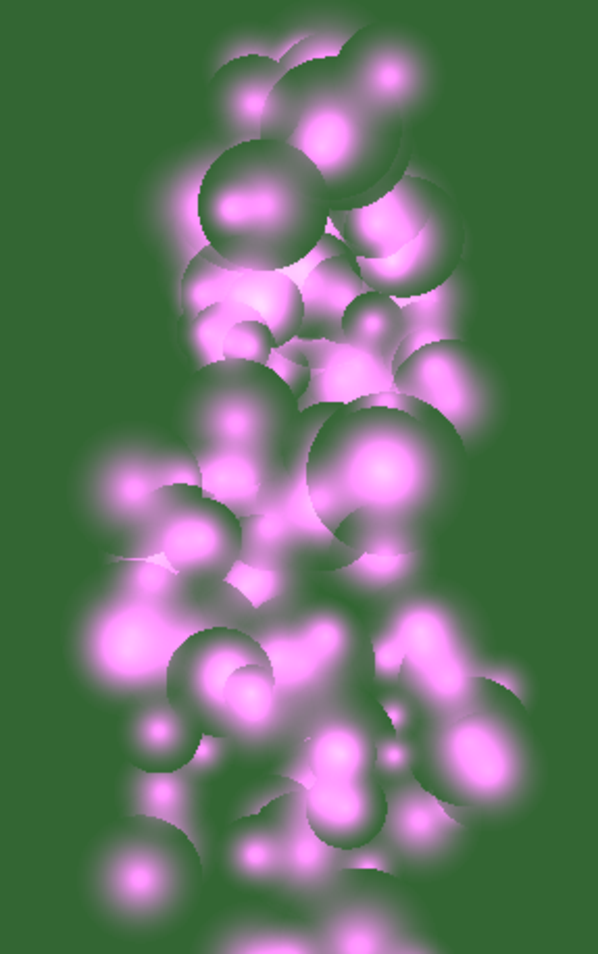
\includegraphics[scale=0.4]{bilder/BlendingEnabled}
\caption{Partikelsystem bei aktiviertem Blending}
\label{fig:BlendingEnabled}
\end{figure}

Abbildung \ref{fig:BlendingEnabled} zeigt wie das Partikelsystem bei eingeschaltetem Blending und Verwendung von {\texttt{glBlendFunc}} mit den Argumenten {\texttt{GL\_SRC\_ALPHA}} und {\texttt{GL\_ONE}} aussieht. Eine Übersicht über die verschiedenen Argumente für {\texttt{glBlendFunc}} und ihre Auswirkungen auf die Farbe eines Fragments ist in \cite{virag:2012} zu finden.

Wie an Abbildung \ref{fig:BlendingEnabled} zu erkennen ist tritt trotz eingeschaltetem Blending der gewünschte Effekt nicht auf. Grund dafür ist der Tiefentest. Für den Tiefentest spielt es keine Rolle, ob ein Fragment teilweise transparent ist, da der Tiefenwert für ein Fragment trotzdem in den Tiefenpuffer geschrieben wird, vorausgesetzt der Wert ist geringer.

Um dies zu umgehen, lässt sich mittels der Funktion {\texttt{glDepthMask}} das Schreiben in den Tiefenpuffer für das Rendern der Partikel verbieten.
Das endgültige Resultat ist in Abbildung \ref{fig:ParticleFinal} zu sehen.

\begin{figure}[h]
	\centering
	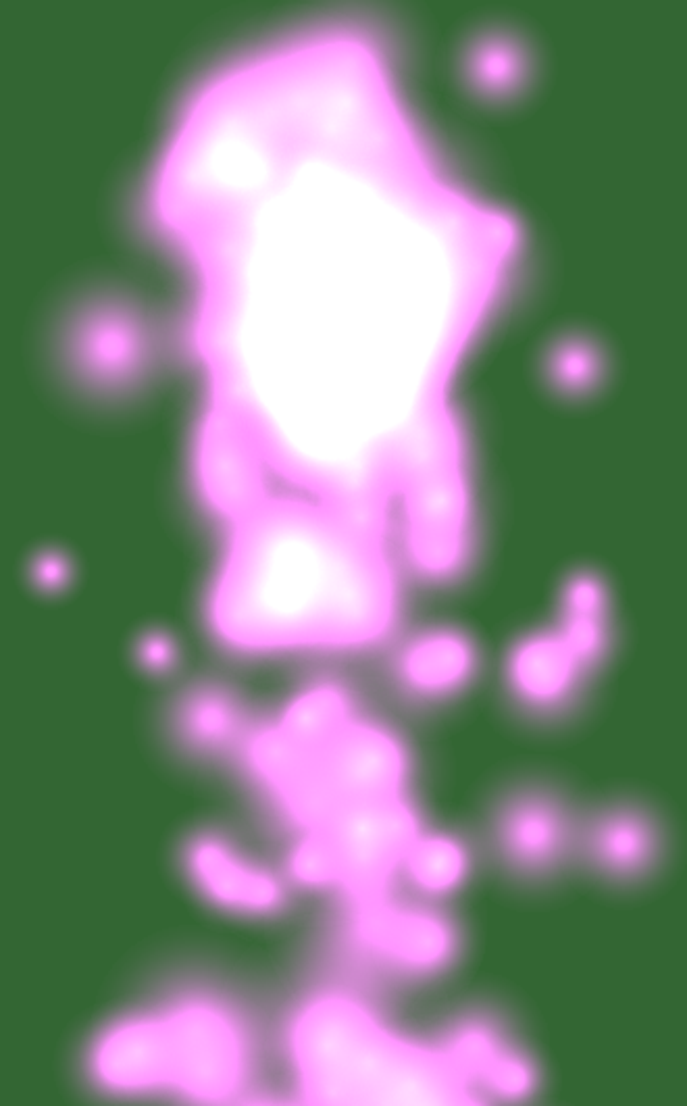
\includegraphics[scale=0.4]{bilder/ParticleFinal}
	\caption{Partikelsystem bei aktiviertem Blending und nicht-beschreibbarem Tiefenpuffer}
	\label{fig:ParticleFinal}
\end{figure}
%


\iffalse
\subsection{Billboarding}
\label{Kapitel_2_-_Unterkapitel_2.4}
%
Für ein besseres visuelles Ergebnis werden die Quads, auf die die Partikeltextur projiziert werden, immer orthogonal zur Blickrichtung der Kamera gerendert. Die Quads erfahren durch die
Modelview-Matrix keinerlei Rotationen. Um diesen Effekt, der als Billboarding bezeichnet wird, zu erreichen muss der Rotationsanteil der View-Matrix, also die linke obere 3x3-Matrix, auf die Einheitsmatrix gesetzt werden.

(Hier Abbildung ohne Billboarding)

Rotationsmatrizen sind Orthogonalmatrizen, das heißt, dass ihre Inversen ihren Transponierten entsprechen. Es genügt also beim Berechnen der Modelview-Matrix die obere linke 3x3-Matrix der Model-Matrix durch die Transponierte des Rotationsanteils der View-Matrix zu ersetzen. Da die Partikel in unserem System auch eine Größe haben wird die resultierende ModelView-Matrix noch mit einer Skalierungsmatrix multipliziert.
\fi